\newcount\draft\draft=0 % set to 0 for submission or publication
\newcount\cameraready\cameraready=1

\ifnum\cameraready=0
\documentclass[preprint]{sigchi}
\toappear{}
\else
\documentclass{sigchi}
\fi

\ifnum\draft=1
  \newcommand{\Revision}{562f3b1}

  \usepackage{drafthead}
\fi
\usepackage{xxx}

% Use this command to override the default ACM copyright statement (e.g. for preprints).
% Consult the conference website for the camera-ready copyright statement.


%% EXAMPLE BEGIN -- HOW TO OVERRIDE THE DEFAULT COPYRIGHT STRIP -- (July 22, 2013 - Paul Baumann)
% \toappear{Permission to make digital or hard copies of all or part of this work for personal or classroom use is 	granted without fee provided that copies are not made or distributed for profit or commercial advantage and that copies bear this notice and the full citation on the first page. Copyrights for components of this work owned by others than ACM must be honored. Abstracting with credit is permitted. To copy otherwise, or republish, to post on servers or to redistribute to lists, requires prior specific permission and/or a fee. Request permissions from permissions@acm.org. \\
% {\emph{CHI'14}}, April 26--May 1, 2014, Toronto, Canada. \\
% Copyright \copyright~2014 ACM ISBN/14/04...\$15.00. \\
% DOI string from ACM form confirmation}
%% EXAMPLE END -- HOW TO OVERRIDE THE DEFAULT COPYRIGHT STRIP -- (July 22, 2013 - Paul Baumann)


% Arabic page numbers for submission.
% Remove this line to eliminate page numbers for the camera ready copy
\pagenumbering{arabic}


% Load basic packages
\usepackage{balance}  % to better equalize the last page
\usepackage{graphics} % for EPS, load graphicx instead
\DeclareGraphicsExtensions{.pdf,.jpg,.png}
\graphicspath{{./figures/}}
\usepackage{times}    % comment if you want LaTeX's default font
\usepackage{mathptmx}
\usepackage{url}      % llt: nicely formatted URLs

% llt: Define a global style for URLs, rather that the default one
\makeatletter
\def\url@leostyle{%
  \@ifundefined{selectfont}{\def\UrlFont{\sf}}{\def\UrlFont{\small\bf\ttfamily}}}
\makeatother
\urlstyle{leo}


% To make various LaTeX processors do the right thing with page size.
\def\pprw{8.5in}
\def\pprh{11in}
\special{papersize=\pprw,\pprh}
\setlength{\paperwidth}{\pprw}
\setlength{\paperheight}{\pprh}
\setlength{\pdfpagewidth}{\pprw}
\setlength{\pdfpageheight}{\pprh}

% Make sure hyperref comes last of your loaded packages,
% to give it a fighting chance of not being over-written,
% since its job is to redefine many LaTeX commands.
\usepackage[pdftex]{hyperref}
\hypersetup{
pdftitle={draft},
pdfauthor={LaTeX},
pdfkeywords={},
bookmarksnumbered,
pdfstartview={FitH},
colorlinks,
citecolor=black,
filecolor=black,
linkcolor=black,
urlcolor=black,
breaklinks=true,
}

\usepackage{color}
\definecolor{lightgray}{rgb}{0.8,0.8,0.8}

% create a shortcut to typeset table headings
\newcommand\tabhead[1]{\small\textbf{#1}}

\usepackage{xspace}
\newcommand\sys{Arfid\xspace}

\newcommand{\figref}[1]{Figure~\ref{#1}}
\newcommand{\tblref}[1]{Table~\ref{#1}}

\newcommand{\etal}{et~al.\@\xspace}

% End of preamble. Here it comes the document.
\begin{document}

\title{Pointing and Clicking in Space}

\ifnum\cameraready=1
\numberofauthors{2}
\author{
  \alignauthor Edward Zhang\\
  \affaddr{Dept. of Computer Science \& Engineering}\\
    \affaddr{University of Washington}\\
    \email{edzhang@cs.washington.edu}\\
  \alignauthor James Youngquist\\
  \affaddr{Dept. of Computer Science \& Engineering}\\
    \affaddr{University of Washington}\\
    \email{jay@cs.washington.edu}\\
}
\fi % cameraready

\maketitle

\begin{abstract}
3D interaction using the traditional mouse, keyboard and 2D screen is often
challenging and unintuitive, due to the inherently 2D nature of these devices.
Many previous systems have examined the effects of higher degree-of-freedom
input devices and enhanced output devices on 3D task performance. However,
the colocation of input space with perceived output space has not been well
studied. We believe that the alignment of input and output will make the virtual
environment seem real, allowing the full use of spatial intuition.
We present a preliminary study that compares performance on a 3D
point selection task across different input modalities (traditional mouse and
keyboard, a standard 6-DOF wand device, and a colocated free-space method) and
output modalities (traditional 2D display and a stereoscopic, head-tracked 3D
display). The results indicate the superiority of stereoscopic output and
suggest that, while current 3D input technology is still immature, high
degree-of-freedom input devices are not only preferred by users over the mouse
and keyboard, but are also quantitatively more efficient and intuitive.
\end{abstract}


\section{Introduction}\label{sec:intro}
Humans operate in a world of three spatial dimensions, and have developed a
corresponding intuition on interacting with physical objects.  If we see a
coffee mug on a table, we can reach out and grab the mug with absolute
confidence in where our hand is going. Unfortunately, when dealing with
virtual 3D data, most of this intuition is lost. Computer-aided design systems
and 3D modelling software present 3D scenes on 2D screens and require the use
of a keyboard and inherently 2-degree-of-freedom mouse to perform such
complicated tasks as selection, rotation, and viewpoint control. This results
in complicated, unintuitive workflows; for example, the standard method to
move an object in a virtual scene is to decompose a translation into several
planar movements, usually aided by orthogonal projections (front view, side
view, top view). In this paper we investigate methods to make interacting with
virtual 3D data as fluid and natural as interacting with the physical world.

We focus our efforts on examining the input and output devices that are
currently used in 3D user interfaces. Several existing systems have already
attempted to make use of physical intuition by developing high degree-of-freedom
input devices to interact with 3D information \cite{manders2010gesture,
mattheiss2011navigating,mine1997moving}, or depth cues such as
stereoscopy or parallax \cite{boritz1997study, schultheis2012comparison}.
Many of these works include studies showing the superiority (or inferiority)
of the system compared with traditional mouse-and-keyboard systems.

However, these studies focus on only half of the factors relevant for intuition;
visual feedback is rarely adapted to react seamlessly with the input device.
Instead, natural input devices are used to manipulate an onscreen object, which
is very different from intuitively reaching out to the object. In our coffee
mug example, we have to manipulate the mug at the end of a long stick. We
believe that by colocating the 3D interaction space with a 3D display space
with appropriate depth cues, we can recover the intuitive feeling of interacting
with a physical object. Imagine that your mug, physically located on the table
on the other side of the room, was virtually rendered directly in front of you;
you can once again reach out and "grab" it intuitively, as if it was real.

In this paper, we present the results of a preliminary study investigating the
effects of both input and output methods on performance in a 3D point selection
task. Specifically, we compare the standard 2D monitor with orthographic
projections with a stereoscopic, head-tracked output display. We also compare a
standard mouse and keyboard input with a 6-DOF ``3D mouse'' and a free-space
input sensor with a 1-to-1 mapping to the virtual space.

%% mention that we don't do anything with haptics or force feedback?


\section{Related Work}\label{sec:related}
Mixed reality systems often focus on the human hand for natural interaction.
Although several 3D manipulation systems use direct mappings between hand
position and a virtual hand, such as \cite{poupyrev1996go},
comparatively few aim to make the perceived 3D position of the hand proxy be
coincident with the user's natural perception of their
hand location. The relevant perceptual phenomenon, known as {\bf
proprioception}, is a person's automatic knowledge of the position and
orientation of their
limbs relative to themselves. The use of proprioception in 3D interfaces was
investigated by Mine in \cite{mine1997exploiting}, which found that
in an immersive virtual environment, manipulating objects colocated with the
users hand was more efficient than manipulation at an offset. Several systems,
such as \cite{mulder2002personal, prachyabrued2011dropping}, use a two-layered
tabletop with a mirrored display above a physical table; in these systems the
interaction space, underneath
the display and above the table, is directly mapped to what the user sees in the
display. The aforementioned systems are strictly virtual reality systems, since
the actual environments displayed
are still completely synthesized. Recent work by Microsoft Research, the
Holodesk \cite{holodesk}, has instead used half-silvered mirrors to create an
augmented reality
interaction space, where the user can see their hands interacting in the same
world as virtual objects. Holodesk focused on realistic physical interactions
within the space,
representing real objects as point clouds that can knock over or hold up other
objects.

Several works have investigated the effectiveness of novel, high-DOF input
devices for 3D tasks by directly comparing them to traditional devices,
especially the mouse.
Evaluation methods generally involve performing fundamental 3D tasks, especially
selection, placement, and rotation. Input methods are compared based on their
speed and accuracy. The SpaceNavigator, a commercially available high DOF
device, was found to be inferior to the mouse for placement tasks in
\cite{mattheiss2011navigating}. B{\'e}rard \etal also found the mouse to be more
effective than several high-DOF devices for placement tasks
in \cite{study1}.  However, a later study by the same group found that enhanced
visual feedback, in the form of pop-up depth views, greatly enhanced the
effectiveness
of the high-DOF device, and was found to perform better than the mouse
\cite{study2}. Schultheis \etal find the mouse inferior to high DOF input devices
for a docking task consisting of achieving a target placement and orientation
\cite{schultheis2012comparison}.

There have also been works examining the effects of depth cues on 3D task
performance. Wanger \etal examine 2D renderable depth-cues, such as shadows,
background textures, and motion cues, in \cite{wanger1992perceiving}. Boritz and
Booth compare monoscopic and stereoscopic displays, as well as viewpoint
tracking, with subjects using a 6-DOF input device, finding stereoscopic
displays to be superior to monoscopic displays \cite{boritz1997study}. In
contrast, Schultheis \etal found no significant
difference between monoscopic and stereoscopic outputs
\cite{schultheis2012comparison}. The evaluation of the Holodesk
system also involved
a user study, in which they compared performance on a selection task with varying
depth cues. This study
focused on the effectiveness of aligning the location of physical objects in the tabletop
space with the apparent locations of virtual objects. They found that aligned
stereoscopic display systems were better than aligned non-stereoscopic systems
with appropriate occlusion cues, and unaligned displays resulted in the slowest
performance \cite{holodesk}. As far as we are aware, only Schultheis \etal have
simultaneously varied 3D input and output modalities; however they did not
examine direct colocation of input and output spaces as Holodesk did
\cite{schultheis2012comparison}.



% Pictures of input devices?
\section{System Design \& Implementation}\label{sec:design}

Driven by the requirements of the experiment design, we created a testing
platform based on a standard desktop computer, various input devices, a USB
camera, and a 3D stereoscopic monitor.  These components are described in
detail below.

\subsection{Input Devices}
The goal with our input device selection and interface design was to isolate
the characteristics of the input method to be applicable to many types of
device.  Thus our conclusions using the Leap Motion should be transferable to
any in-air, free-hand input mechanism, our conclusions with the mouse should
be applicable to the trackpad, and so on.

While our original inspiration was to compare standard mouse and keyboard
interfaces with 1-to-1 free space interfaces, we recognized that other devices
have been designed and tested for 3D tasks. These include 3D-joystick analogs
such as the SpaceNavigator \cite{mattheiss2011navigating}; 6-DOF tracked
wand-based systems that function in relative space rather than absolute space,
such as the Wiimote or Razer Hydra; and paired input devices to be used by both
hands simultaneously such as the DepthSlider \cite{study1}. To limit the length
of our experiment we elected to investigate only the wand-based 3D relative
input devices in addition to the mouse interface and the aligned free-space
interface.

For each input device, we also considered the particular interactions
experiment participants would perform. In particular, we decided to evaluate
performance on a 3D selection task with only three degrees of freedom (see
prior section) rather than a docking task that involved position and
orientation, which would require six degrees of freedom. We also did not allow
users to control the viewpoint beyond head tracking. These decisions were made
to preserve the ``purity'' of our input device evaluation, since while
intuitive mappings from input device movement to 3D position are fairly
obvious and are arguably implied by the device design, camera control
movements and arbitrary rotational movements are much less so.

For our task, each input device needs to two things: {\it point}, specifying a
point in the 3D space, and {\it click}, indicating acceptance of the current
point. We refer to {\it relative} and {\it absolute} input devices, where
absolute input devices have a direct 1-to-1 spatial relationship with the
virtual space (i.e.\ a rotation, uniform scaling, and translation maps virtual
space to real world space) while relative input devices preserve directions
but may map magnitudes of motions non-linearly. Standard mice and touchpads
are relative, not absolute, since faster movements across the same physical
distance map to larger mouse pointer movements. A device such as a trackball
or joystick is neither relative nor absolute, since they don't move spatially.

\subsubsection{Mouse and Keyboard (2D Relative Interface)}
Our mouse and keyboard interface mimics the input mechanisms used in standard
3D modelling software. To achieve precise arbitrary spatial positioning, the
standard interaction involves several orthogonal projections in subwindows
(containing a top view, side view, and front view). The mouse can be used to
drag an object in each of the orthogonal projections (within a single
axis-aligned plane) to its final position.

We streamline this interaction by allowing the user to change the plane of
interaction by holding down the Shift key. By default the mouse moves in the
plane parallel to the screen, the same mapping used by the 2D WIMP interface;
holding shift switches to moving in the plane parallel to the desk, the same
plane as the mouse movement. This eliminates the overhead involved with
switching the mouse from subwindow to subwindow and the added clutch
interaction \cite{bravenuiworld} necessary to differentiate mouse pointer
movement and 3D translation.

Fortunately the mouse is already a point-and-click device, so we reuse the
left mouse button as our {\it click} input.

\begin{figure}
    \centering
    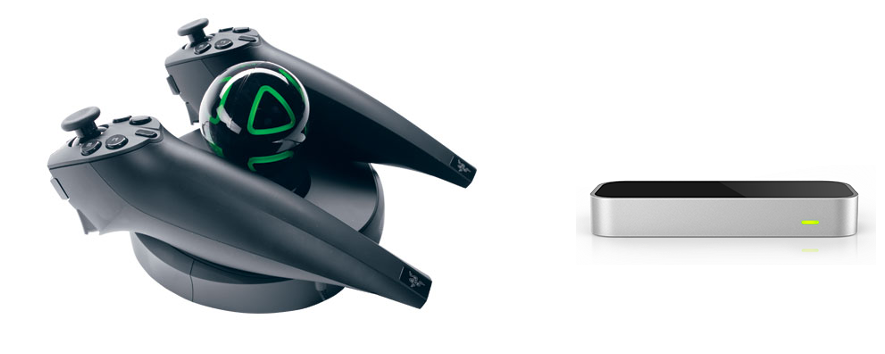
\includegraphics[width=\columnwidth]{input.png}
    \caption{Input Devices: Left: Razer Hydra. Right: Leap Motion. Device sizes
        not to scale.}
    \label{fig:input}
\end{figure}

\subsubsection{Razor Hydra (3D Relative Interface)}
We implement the 3D relative interface using the Razer Hydra
(\figref{fig:input}). We reuse the
conceptual model of the mouse with this interface, where the movement of the
device has a direct but not 1-to-1 mapping with the movement of a cursor (hence
relative interface). Therefore, we also refer to the Hydra interface as the 3D
mouse.

The Hydra is a magnetically tracked 6-DOF input device. It tracks position and
orientation of two wands relative to a base station. Each wand includes a thumb
joystick, 2 trigger buttons, and several thumb buttons. For our task, we use
only one of the two wands. We use one of the thumb buttons as a clutch; we
translate the cursor appropriately only if the clutch is pressed. This allows a
similar interaction to the mouse, where the user can pick up the mouse and move
it if they have reached a limit of its operational area. We use one of the
trigger buttons to do our {\it click} interaction.

Unfortunately, the magnetic tracking of the Hydra makes it fairly vulnerable to
magnetic fields such as those produced by large electronics; this meant that it
was ill-suited as a registered absolute input interface.

\subsubsection{Leap Motion (3D Absolute Interface)}
We implement the 3D absolute interface using the Leap Motion
(\figref{fig:input}). The device uses
infrared light using a proprietary method to model the spatial positions of
human hands. We chose to use the Leap instead of more common
RGBD cameras because of its compatible operating range, low latency and high
data rates.

The precision of the Leap allows us to track a fingertip as the cursor
position.  We sense cursor movement only when a single finger on a hand is
extended. The primary reason is to provide a simple reset mechanism if the
Leap mistracks the finger. We use the keyboard spacebar to perform the
{\it click} interaction, since hand-only gestures are often noisy with the Leap
or interfere with precise 3D placement.

Unfortunately, the Leap technology is still immature. It is sensitive to
ambient infrared light, and its model-based tracking is imperfect and often
loses track of users. This resulted in very high variability in the
performance of the device. In further experiments we anticipate testing
alternate absolute free-space input devices.

\subsection{Output Devices}
Similar to our input devices, we aimed to have the output interfaces as simple
as possible to generalize across particular application outputs. Our main test
scene consists of a few simple elements: two targets in the shape of
spaceships, a cursor element in the shape of an icosahedron, and a grid placed
at approximately screen depth as a reference element.

We provide minimal feedback for depth when rendering, since we want to
specifically measure the benefits of stereoscopic and parallax depth
cues. Thus we did not provide shadows or additional helper indicators of
position. We do, however, highlight the target element if the cursor is within
clicking range; we found that this helped in many situations including with
the quarter-sized 2D subwindows, when objects were occluded, and when subjects
had difficulty with stereopsis. Finally, we change the color of the cursor
depending on whether the clutch was enabled (and the cursor tracked). This
primarily helped the Leap input interface, which would sometimes lose track of
the user's hand.

\begin{figure}
    \centering
    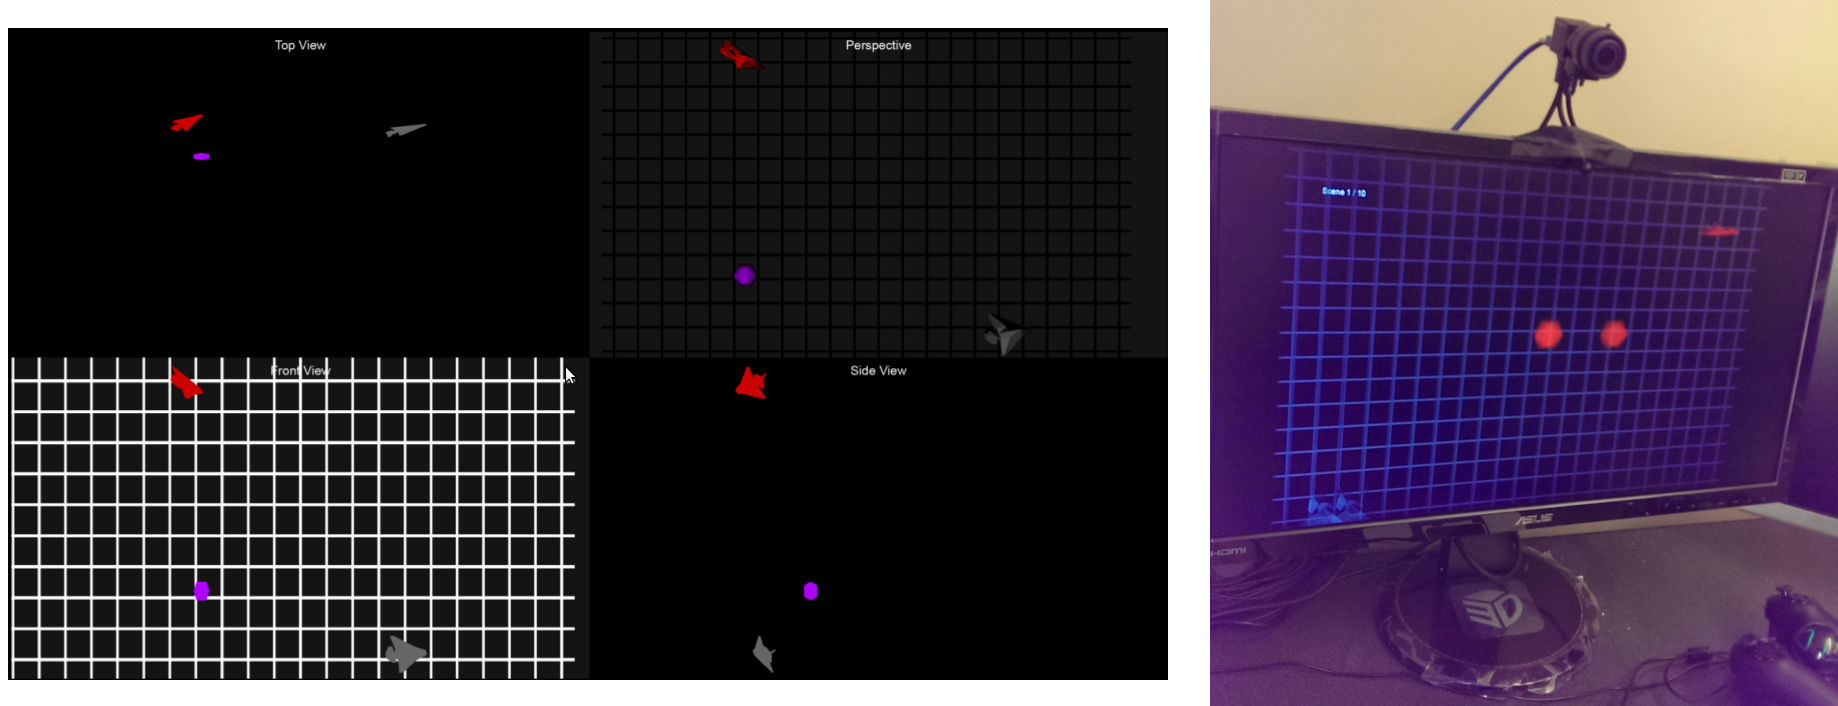
\includegraphics[width=\columnwidth]{displays.png}
    \caption{Output modalities: {\bf Left}: 2D split-screen output. {\bf Right}:
    3D stereoscopic output. Note the apparent doubling of objects on screen;
when wearing shutter glasses each eye will see one of the images.}
    \label{fig:output}
\end{figure}

\subsubsection{2D Display}
As described above, we use the split-screen orthographic projections commonly
used in 3D modelling software. This consisted of a perspective projection on
the top right, a top view on the top left, a front view on the lower left, and
a side view on the lower right (see \figref{fig:output}). We expect that most
users would focus on the left two displays when using the mouse input, since
those correspond directly with the planes that the mouse moves in.

\subsubsection{3D Stereoscopic Display and Headtracking}
To achieve stereoscopic rendering, we used Nvidia's 3D Vision Automatic
technology \cite{nvidia3dvision}. The hardware we used was an Nvidia GTX580
graphics card, an Asus VG278HE monitor, and a set of wired Nvidia 3D Vision
glasses. The 3D vision monitor displayed images at 120Hz, while the shutter
glasses alternately blocked each eye in a synchronized fashion so that alternate
frames were seen by the left and right eyes (see \figref{fig:output}). While
the technology did not permit full control of rendering in each
eye, we were able to render spatially accurate locations in front of the
monitor given a head position and eye separation, assuming no head roll.

Stereoscopy alone is insufficient to present a convincing 3D scene.  Humans
rely significantly on motion parallax as a depth cue \cite{parallax}, as well
as expecting that percieved visual motion will match accelerations sensed by
the inner ear.  Even while sitting ``still'' people make continous small head
motions.  Without constantly adjusting the virtual camera from which the scene
is rendered to match these motions, even a stereoscopic display will assume a
flat dimension.

To perform head tracking, We used the Aruco augmented reality tracking library
\cite{aruco} to track the location of a fiducial marker (AR tag) placed above
the 3D Vision glasses.  The rectified image stream to Aruco was generated by a
Point Grey Flea3\footnote{\url{http://ww2.ptgrey.com/USB3/Flea3}} camera at
60Hz.  Low pass filtering was applied to the output head positions to reduce
noise that initially led to a vibrating appearance on scene objects.

\subsection{Calibration}

Our system needs to integrate data from up to three separate frames of
reference:

\begin{description}

\item[display space] the 3D graphics rendering space, left handed, with origin
  at the center of the computer monitor.

\item[camera space] a right handed space at the optical center of our head
  tracking camera in which poses from fiducial markers are generated by Aruco.

\item[input space] the frame of reference for the currently selected input
  device.  For the relative input devices (mouse, Hydra) this is essentially
  the same as the display space.

\end{description}

In order to successfully colocate the 3D interaction space with the 3D display
space (Leap with 3D headtracking), we need to have accurate transforms between
the different frames of reference.  Note that head tracking alone only
requires approximate registration to generate believable parallax, and the
relative input devices do not require explicit registration, only dimensional
scaling. The three spaces were registered via the Aruco library also used for
head tracking.

To register the camera space with the display space we placed an AR tag in the
center of the screen and suspended four others at random locations such that
no four of the five tags were coplanar, see \figref{fig:calib1} (which shows
Aruco detected tags as an overlay).  The suspended tags were double sided so
that they could be seen from both the monitor mounted USB camera and a
handheld camera.  Four images at different angles were taken using the
handheld camera, and one was taken from the statically mounted USB camera.  We
used Aruco generated pose information (position and orientation) from each
suspended tags visible to both cameras to compute a transformation chain
between the camera space and the display space.  The final transform to map
from the camera space to the display space was an average of each of these
individual transforms.  Averaging is required due to noise in Aruco's
estimates as a result of quantization errors in the pixel based detection
process.

\begin{figure}
    \centering
    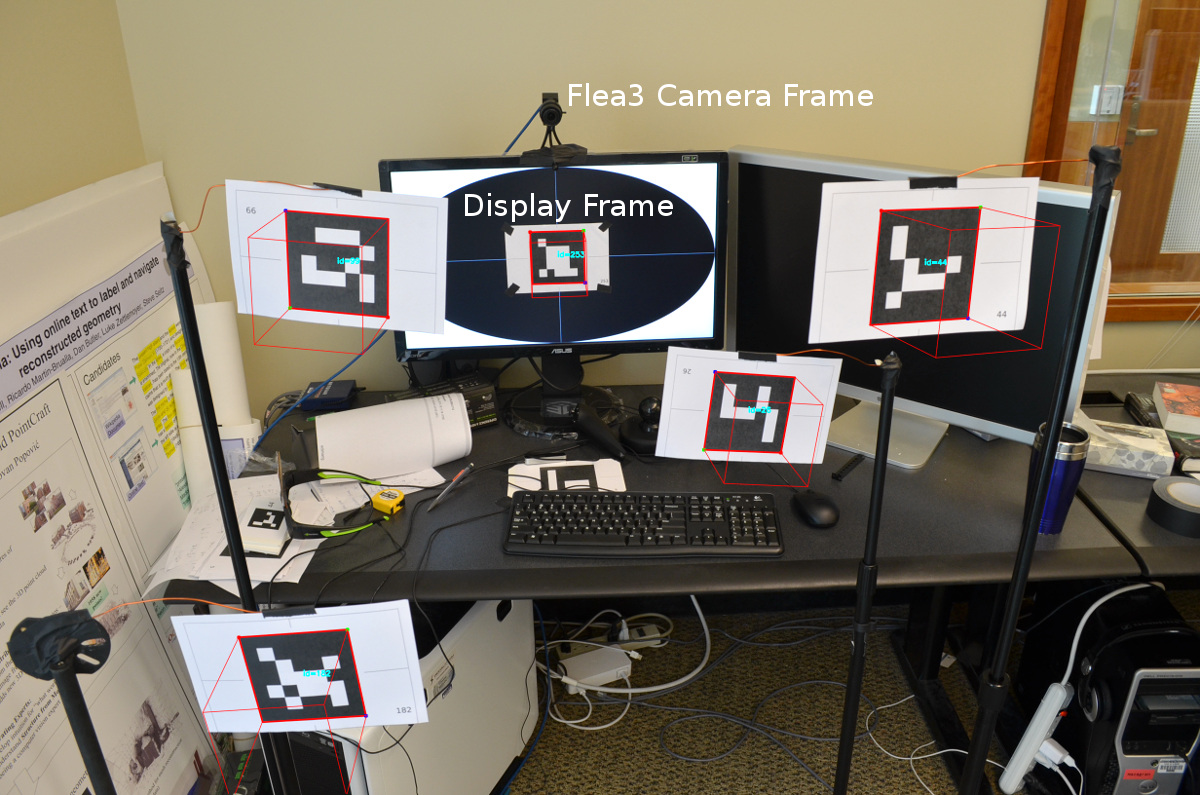
\includegraphics[width=\columnwidth]{calib1.jpg}
    \caption{Display - Camera registration setup}
    \label{fig:calib1}
\end{figure}

Registering the Leap input space with the display space follows a similiar process, see \figref{fig:calib2}.

\begin{figure}
    \centering
    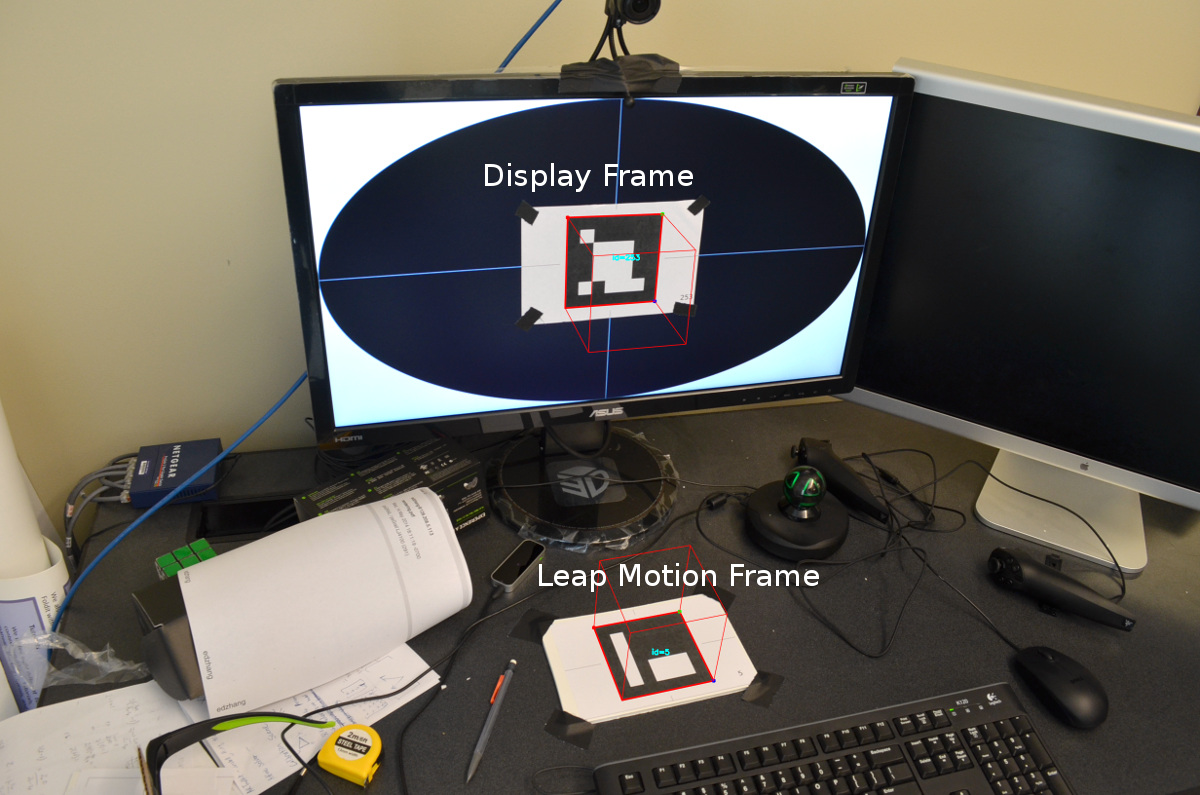
\includegraphics[width=\columnwidth]{calib2.jpg}
    \caption{Display - Input registration setup}
    \label{fig:calib2}
\end{figure}

As a result of this automatic calibration process, we were able to
successfully colocate coordinates in the Leap space with the display space.
Because of limitations in the Leap hardware, such as nonlinearities in the
reported finger location, we implemented per-user tweaking functionality to
achieve adequate colocation over most the input space.


\section{Experiment Design}\label{sec:experiment}

The most basic meaningful interaction task with a display is to place a cursor
on a target region and ``click'' it to indicate activation intention.  Since
this study was intended to evaluate the efficiency differences in input/output
modalities, we limited it to the most basic ``point and click'' operation
possible: two targets are displayed on the screen at random points along with
a cursor.  The \emph{start} target is initially red and when the user
successfully clicks on it, it turns grey and the \emph{end} target becomes
red.  In the following we refer to each pair of start and end clicks for a
given input/output combination as a \emph{trial}.

Even though real world applications that deal with 3D data often involve dense
scenes with occlusion, it is the authors' anecdotal experience that scenes are
transformed (rotated and translated) by a user prior to interaction in order
to make the desired interaction points congruent with the plane of the screen.
This is equivalent to aligning the axes of the points' principle components
with the screen, which maximizes the accuracy of an input device and the
projected resolution in pixels.  Therefor, we limited the target points to be
randomly generated near the surface of a truncated sphere, such that they were
approximately aligned to the plane of the screen.  This means there is no
occlusion and that the euclidean distance between target points is nearly
constant across all trials.  Randomizing target locations is employed to
prevent motor learning effects as a confound.

We recruited 13 individuals to test on the platform described in section
\ref{sec:design}, of which 11 provided suitable data: the first subject
revealed flaws in our test setup, invalidating his results, and another did
not complete the study.  All of the subjects except one are either current
students or professoinals in STEM fields.  Of those whose data was used, the
average age was 26 with 14.6 years of computer use, and 6 were female, 5 male.

Each subject was given a pre-experiment survey (summarized in
\figref{fig:pre_likert}) to ascertain prior familiarity with 3D systems and
interaction, and a post-experiment survey (dicussed further in
\ref{sec:feedback}) to provide feedback on the performance and feel of our
test system.  From the pre-survey we see that even though all the subjects are
familiar with computing systems, that their level of experience with 3D
systems and interaction uniformly ranges the gamut from little-to-none
(e.g. has seen the occasional 3D movie or played a video game set in a 3D
world) to highly (e.g. has much experience in 3D design).

\begin{figure}
    \centering
    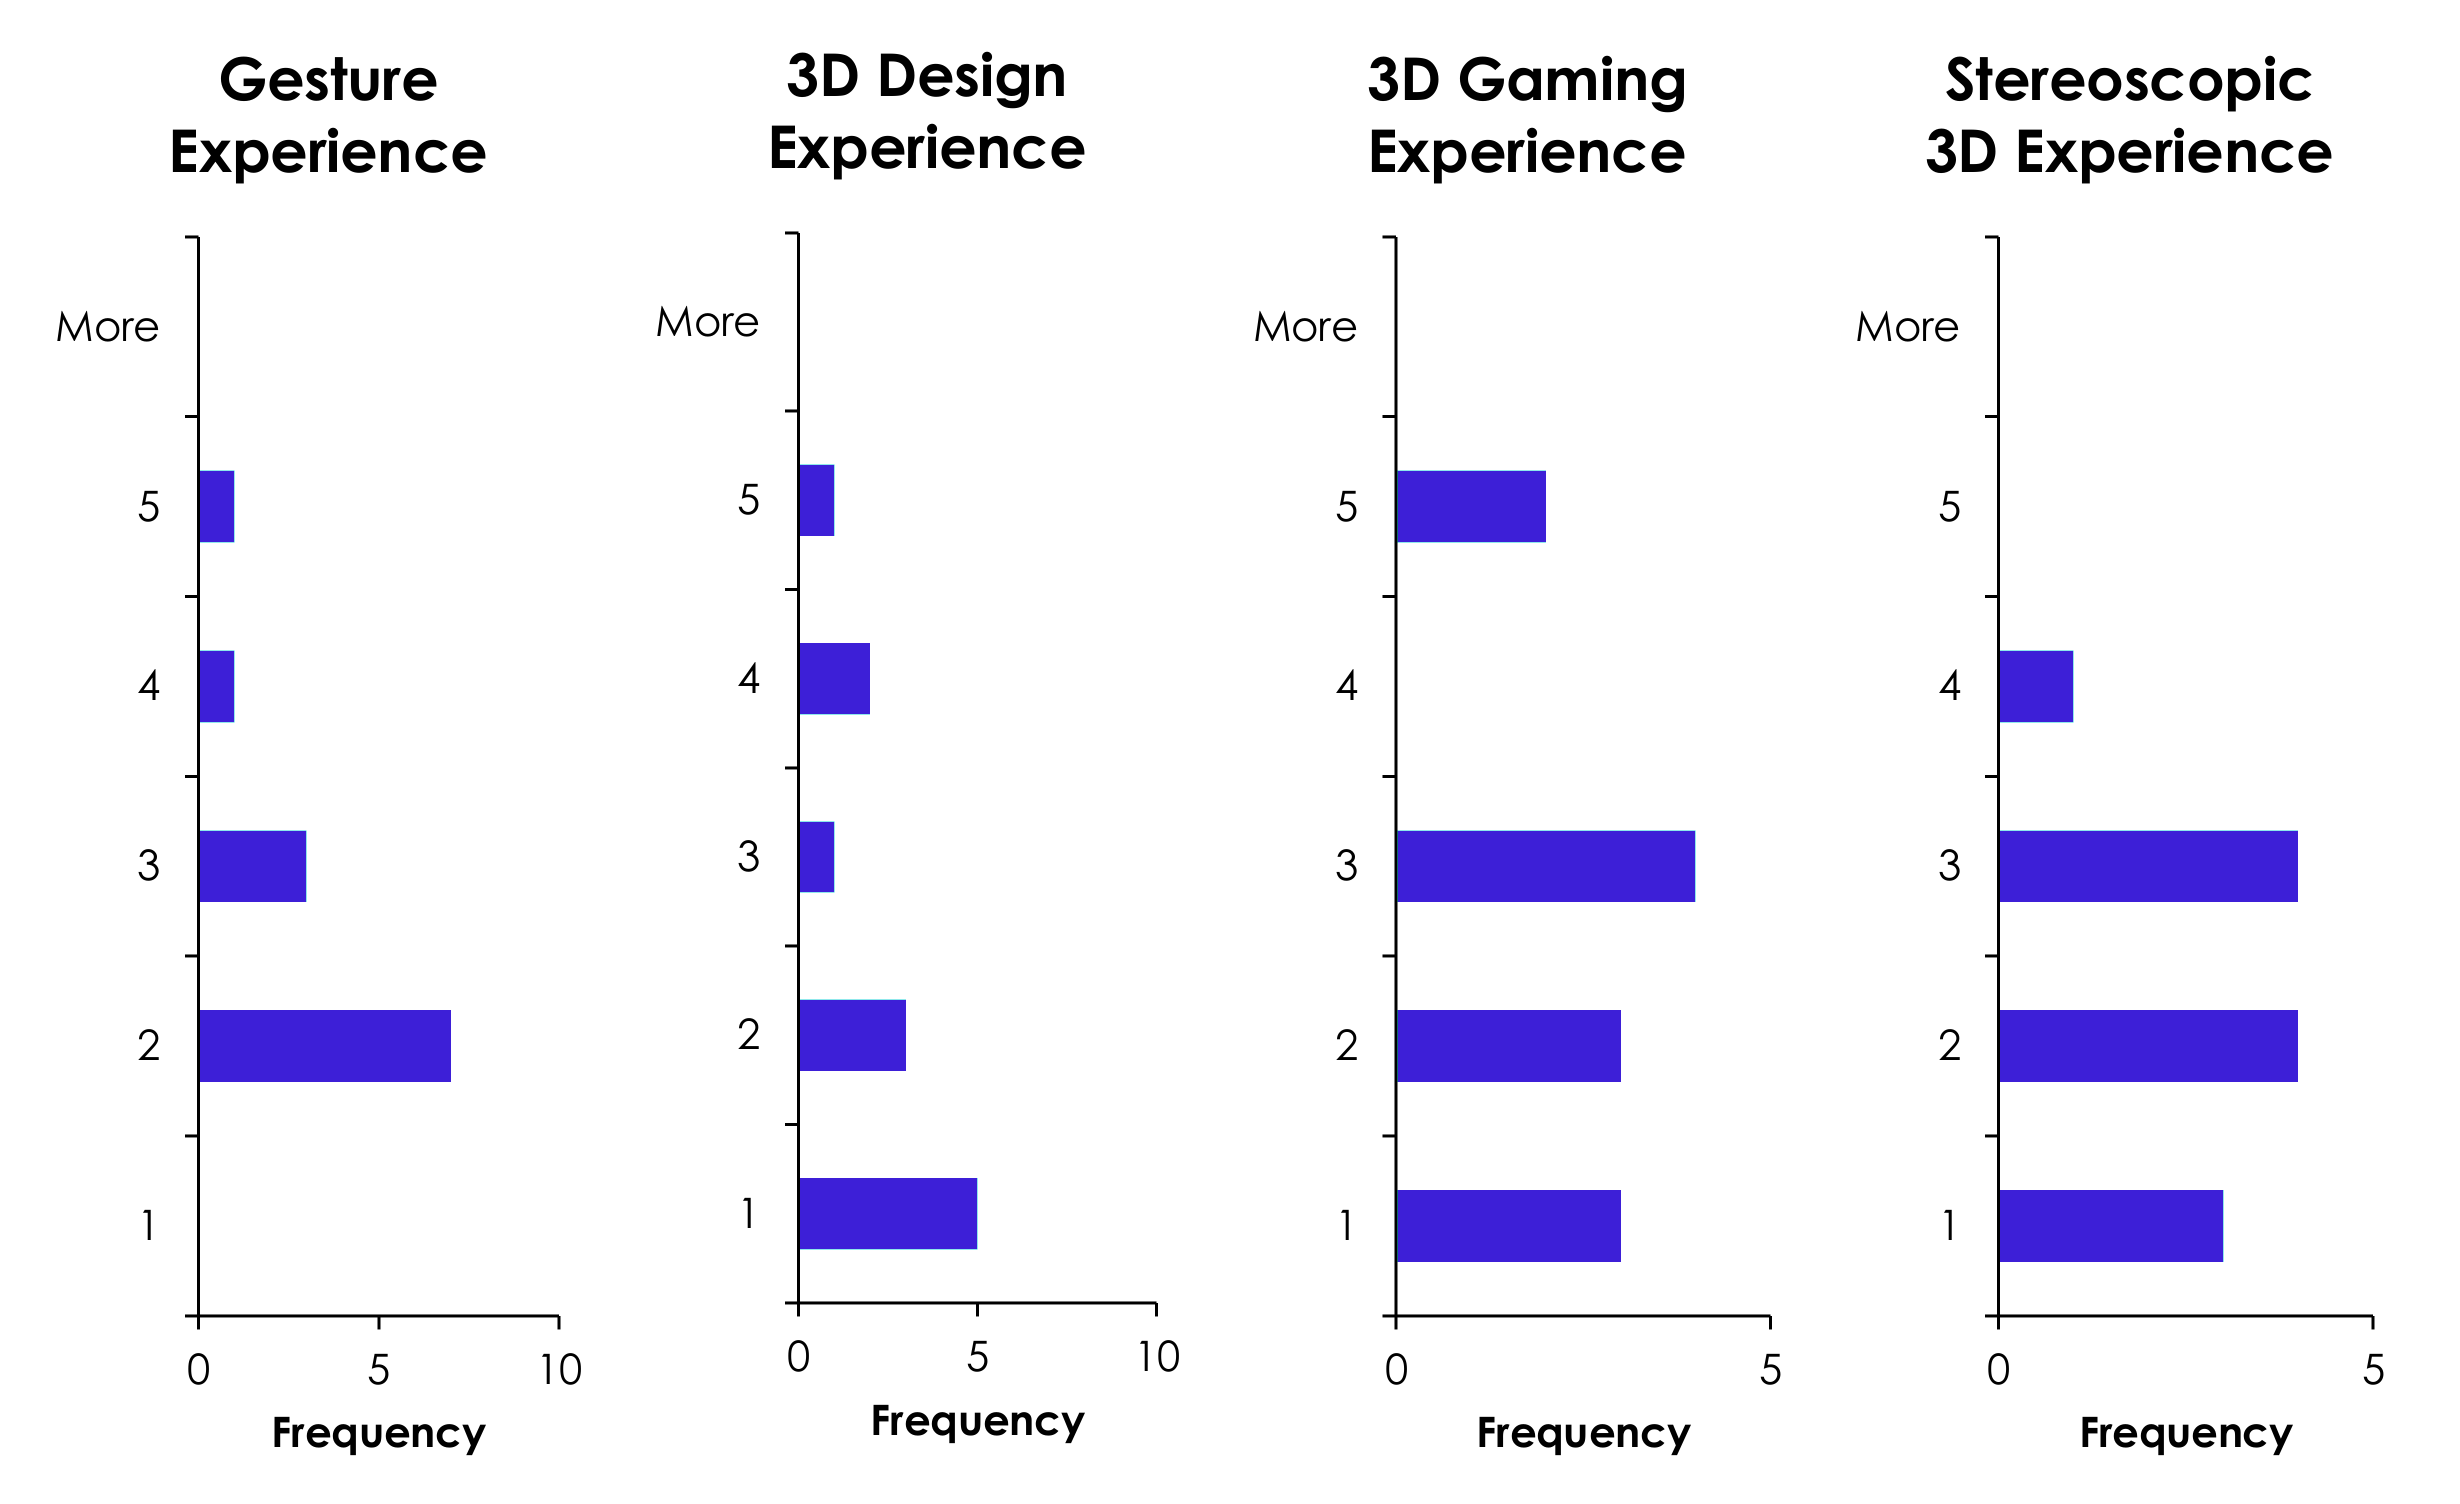
\includegraphics[width=\columnwidth]{pre_likert.png}
    \caption{Pre-experiment responses}
    \label{fig:pre_likert}
\end{figure}

This study was a within-subjects 3x2 design where the input factor has levels
\{Mouse and Keyboard, 3D Mouse, Leap\} and the output factor has levels \{2D
Projections, 3D Headtracked\}.  Each subject was asked to complete 20 trials
for each of the six input/output combination, divided into 12 sessions of 10
trials each.  We used a Latin Square to vary the order of the 12 sessions for
each subject to minimize learning effects from one input/output modality
affecting another.  Prior to starting the 120 trials, each subject was given a
two trial tutorial for each modality.  Subjects were not required to complete
all trials and were informed that they could stop at any time, though only one
chose to stop early (at the halfway point) due to time constraints.  Total
time spent per subject including answering the surveys was around 40 minutes.

We logged cursor pose (3D position and orientation) for each trial at 30Hz for
the duration between clicks on the start and end targets.



\section{Results}\label{sec:results}

\subsection{Completion Time Analysis}\label{sec:timing}
To determine whether input or output interfaces affected performance on the
task, we performed a Repeated Measures ANOVA on the completion times.
Mauchly's test indicated that the assumption of sphericity had been violated
for the Input factor ($\chi^2(2) = 7.218, p = 0.027$), therefore degrees of
freedom were corrected using Greenhouse-Geisser estimates of sphericity
($\epsilon = 0.627$).

\begin{figure}
    \centering
    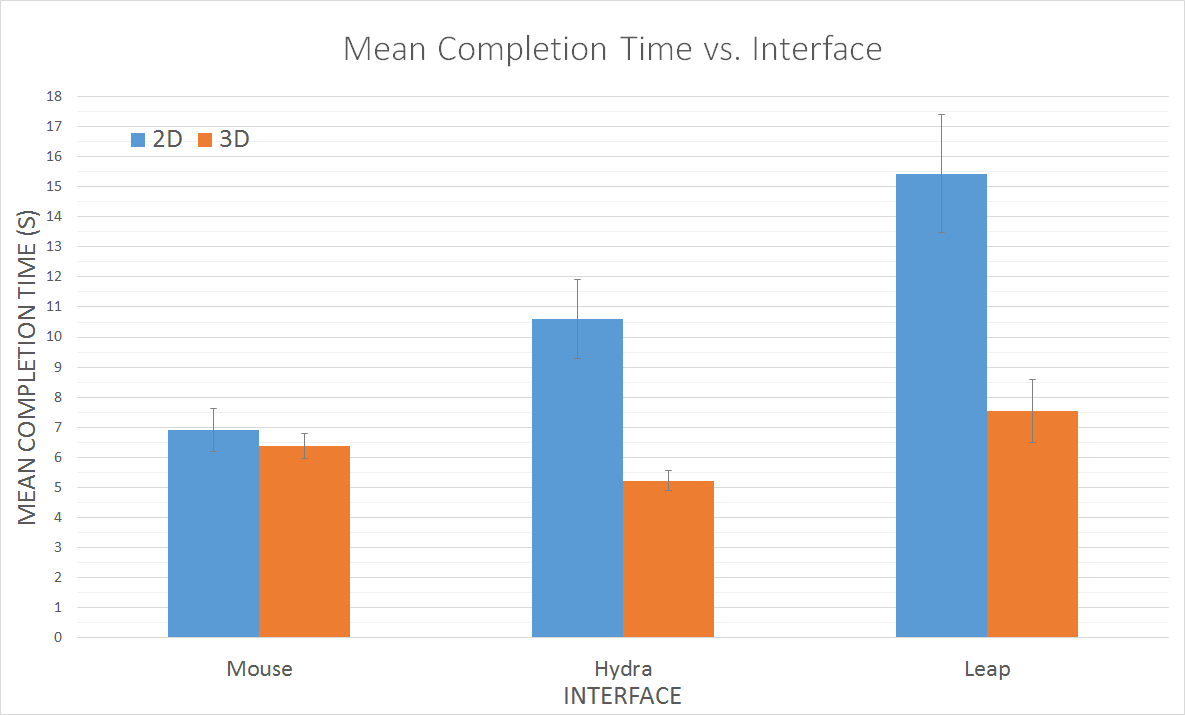
\includegraphics[width=\columnwidth]{timingmeans.png}
    \caption{Mean task completion times for each interface combination}
    \label{fig:means}
\end{figure}

The Repeated Measures ANOVA showed a strong main effect on task
completion time of Input ($F(1.25,11.2) = 8.94, p = 0.009$) and Output ($F(1,9)
= 36.8, p < 0.001$). This was qualified by an interaction between Input and
Output ($F(1.299,) = 11.6, p = 0.004$). \figref{fig:means} shows the means
of per-task completion times with 95\% confidence intervals.

From this data, we see that using the 3D stereoscopic output improved
completion times regardless of input interface used. The fastest input device in
the 2D output case was the mouse, while the Hydra resulted in the fastest mean
completion time overall when used with the 3D stereoscopic output (mean
completion time of $5.22$s).
We note that output interface did not improve performance with the mouse
($6.901$s vs. $6.370$s) as much as with the other two interfaces.

\begin{figure*}
    \centering
    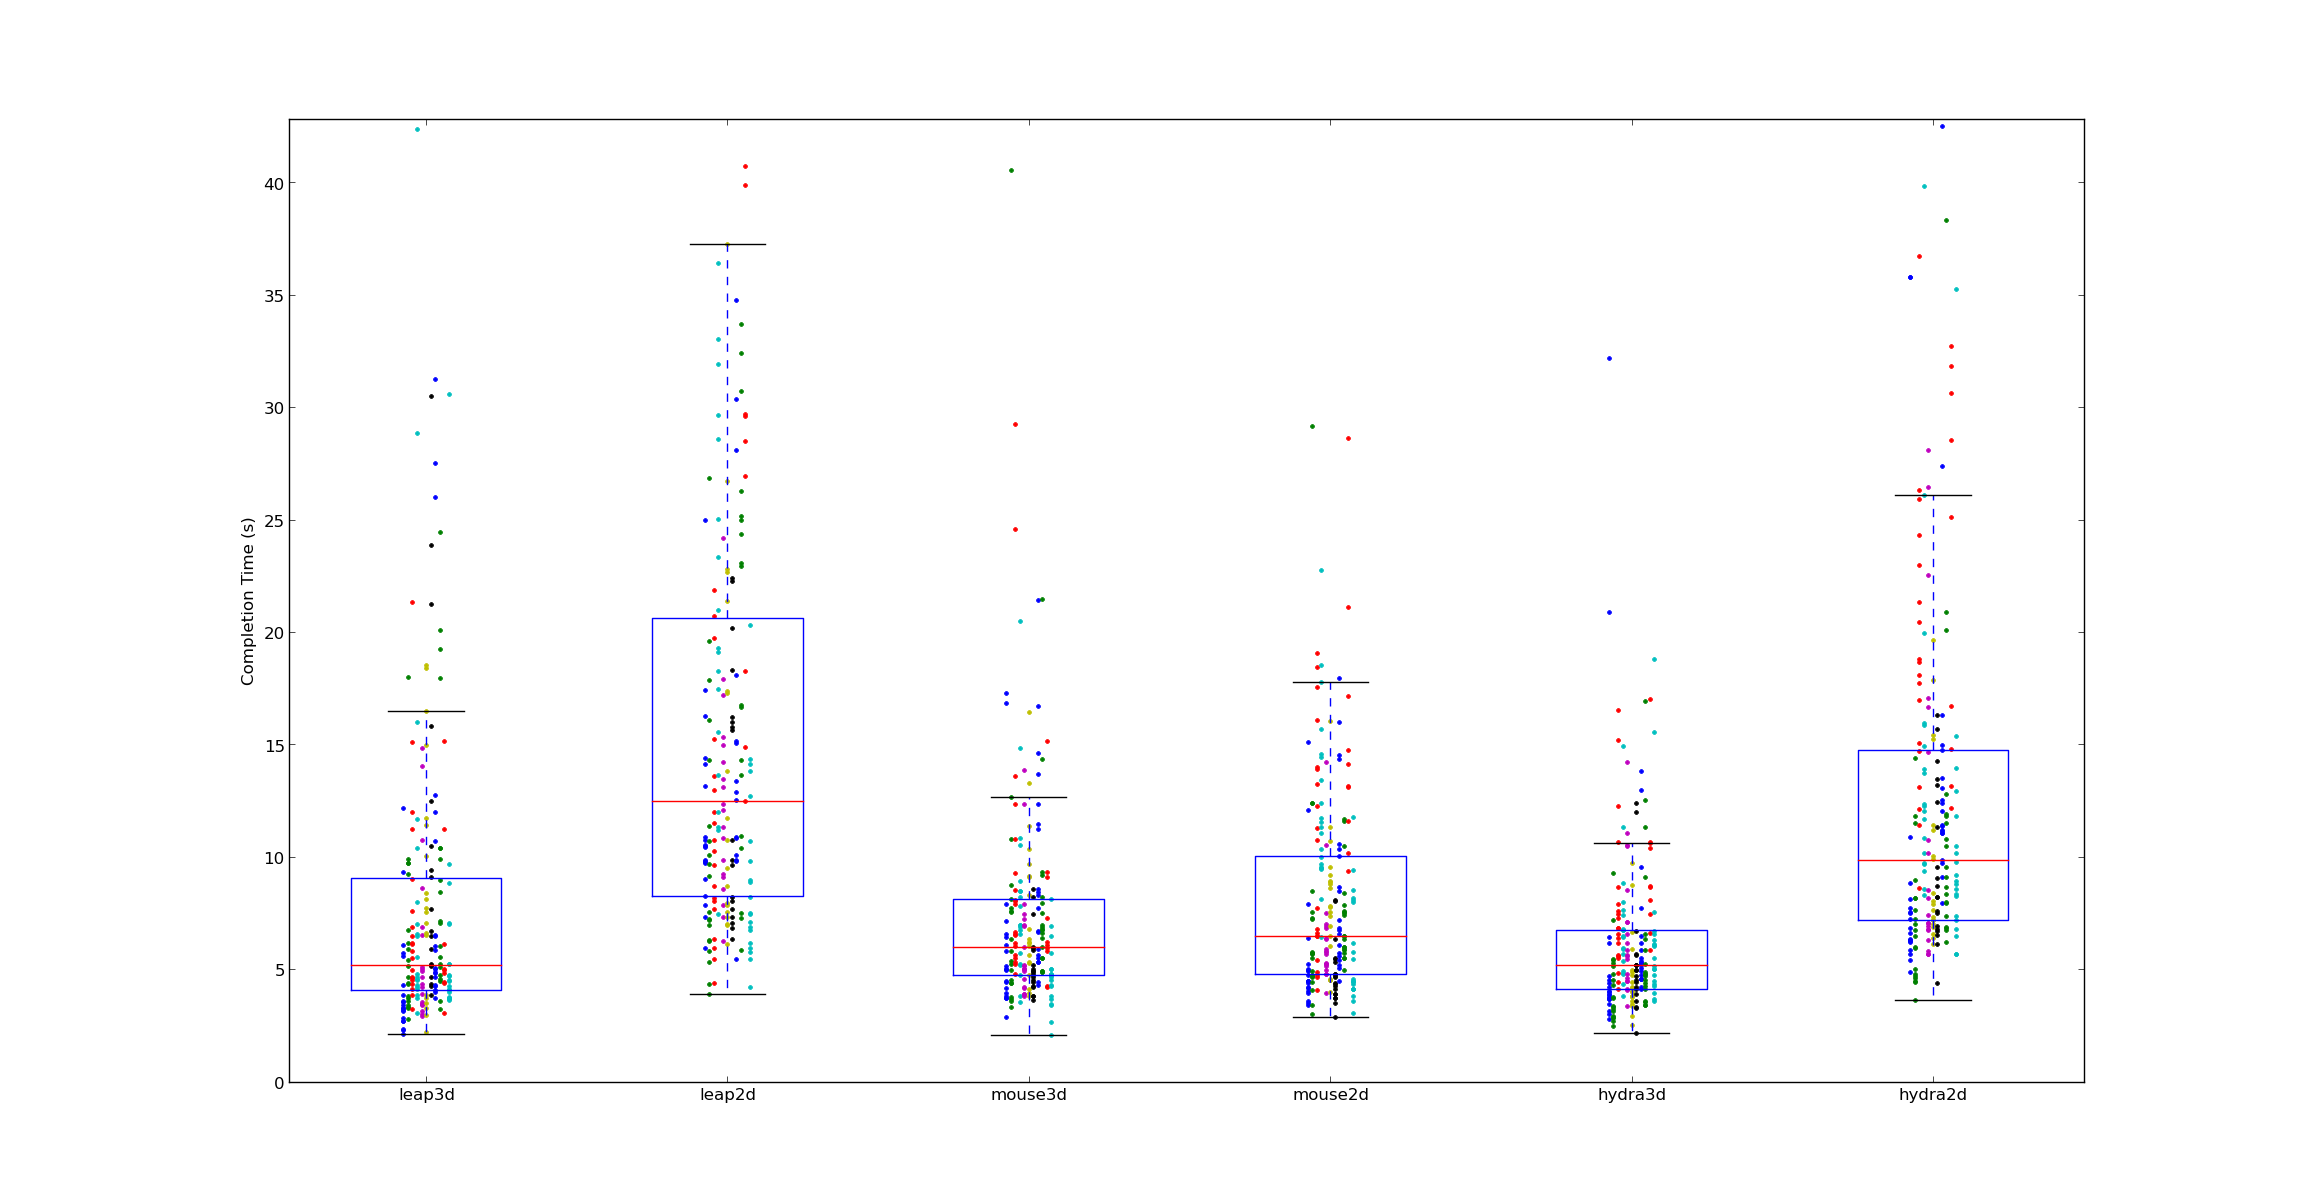
\includegraphics[width=\textwidth]{rawdata.png}
    \caption{Raw completion time data grouped by interface combination.
             Note that there are several outliers in the {\tt leap2d} that
             are outside the bounds of the plot.}
    \label{fig:rawtimes}
\end{figure*}

However, examining the raw data (\figref{fig:rawtimes}) shows that
the Leap had a particularly skewed distribution of completion times.
Using the median as a more robust measure of central tendency, we see
that using the Leap with the 3D output interface had comparable completion
times (median 5.20s) with the Hydra with 3D output (median 5.17s), the
fastest input device; in contrast the median time for the mouse and 3D output
interface was much higher (median 5.98s).

Observing participants during the experiment and reviewing post-experiment
surveys suggest that the Leap's long tail of high completion times occurs
primarily because of the Leap's tendency to lose track of the user's hands.
The Leap technology is still in development, so these results suggest that
performing this experiment with more robust in-air one-to-one input
system would yield more reliable results.


\subsection{Trajectory Analysis}\label{sec:trajectory}

Though the completion time analysis indicates that Hydra / 3D headtracked
combination results in the fastest mean completion time, it possible to derive
insights from visualizing the data itself, in aggregate and on a per subject
basis.  These analyses are subjective.  In the following, all input data were
normalized so that the start target is at the origin and the end target lies
on the positive $x$-axis.

\figref{fig:compressedtracks} shows the tracks for each input/output
combination. Each path is data from a trial; green indicates a trial
completion time of less than 10 seconds and red is over 10 seconds.  Each
point was rotated around the $x$-axis so that it lies on the XY plane,
discarding Z information while minimizing angular distortion.

\begin{figure}
    \centering
    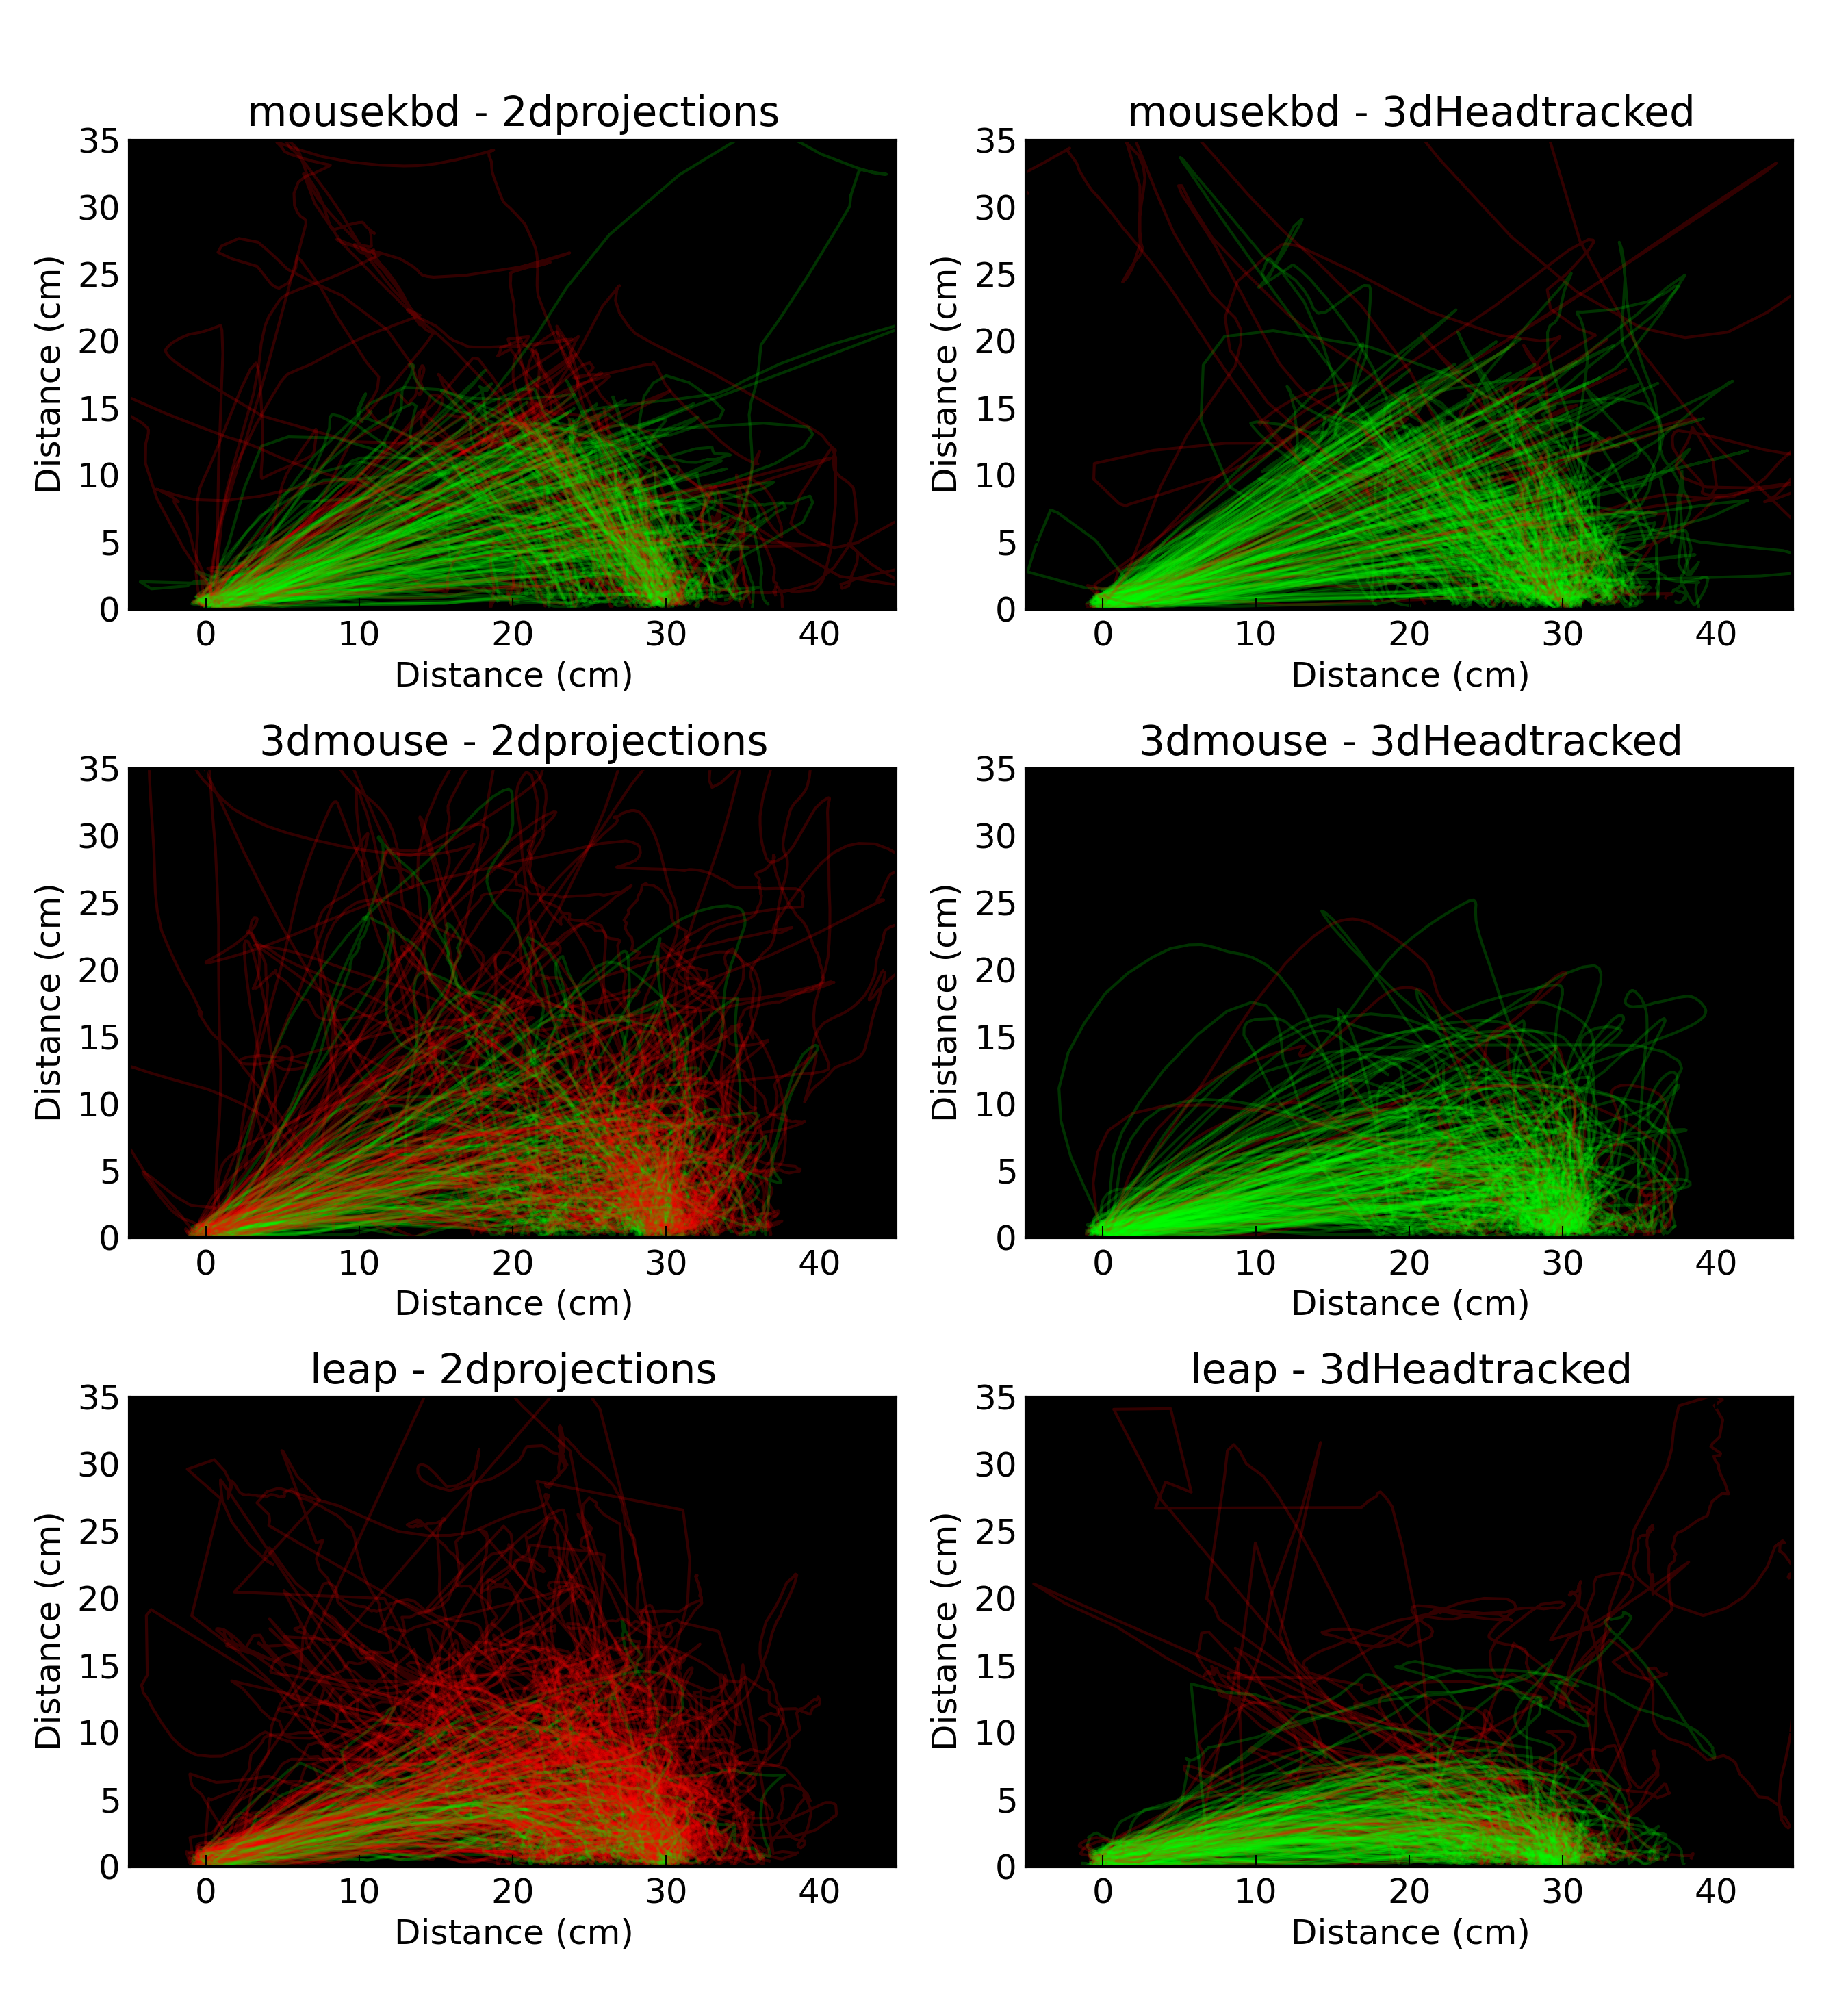
\includegraphics[width=\columnwidth]{paths.png}
    \caption{Cylinder compressed tracks}
    \label{fig:compressedtracks}
\end{figure}

We can see that subjects adopted similar strategies for the mouse and keyboard
regardless of the display type: straight line movements in orthogonal planes.
Orthogonality can't be avoided, but this shows that skills developed in
traditional 2D displays readily transfer.  That is, though the mouse is a
relative positioning input device, users have good mouse-eye coordination that
allows them to quickly reposition the cursor on a plane using mostly straight
line motions.

The straight-line orthogonal movement strategy is also somewhat evident for
the 3D mouse and Leap in the 2D projection case, but their tracks are more
organic looking.  From observing the subjects we noticed that, especially for
the 3D mouse, 3D inputs in the 2D projection case were unintuitive for most
subjects, but that after even the 20 trials conducted, they were able to learn
a decent mapping from hand motion to cursor motion.  See for example
\figref{fig:improvementtimes}.

\figref{fig:improvementtimes} which shows the average reduction in completion
time between the first 3 trials of 20 for an input/output combination, and the
last 3.  We interpret a small reduction as meaning not much learning had to or
could take place to saturate proficiency (median close to zero), whereas a
large reduction (median far from zero) is indicative of an \emph{unintuitive}
input modality.  For example, subjects did not tend to get much better using
the mouse and keyboard, irrespective of output type (saturated prior
experience), nor on the Leap in the 3D headtracked case (intuitive), but they
did improve quite a bit on the 3D mouse in the 2D projections case
(unintuitive).  Note that positive times are partially due to noise induced by
the random target positioning

\begin{figure}
    \centering
    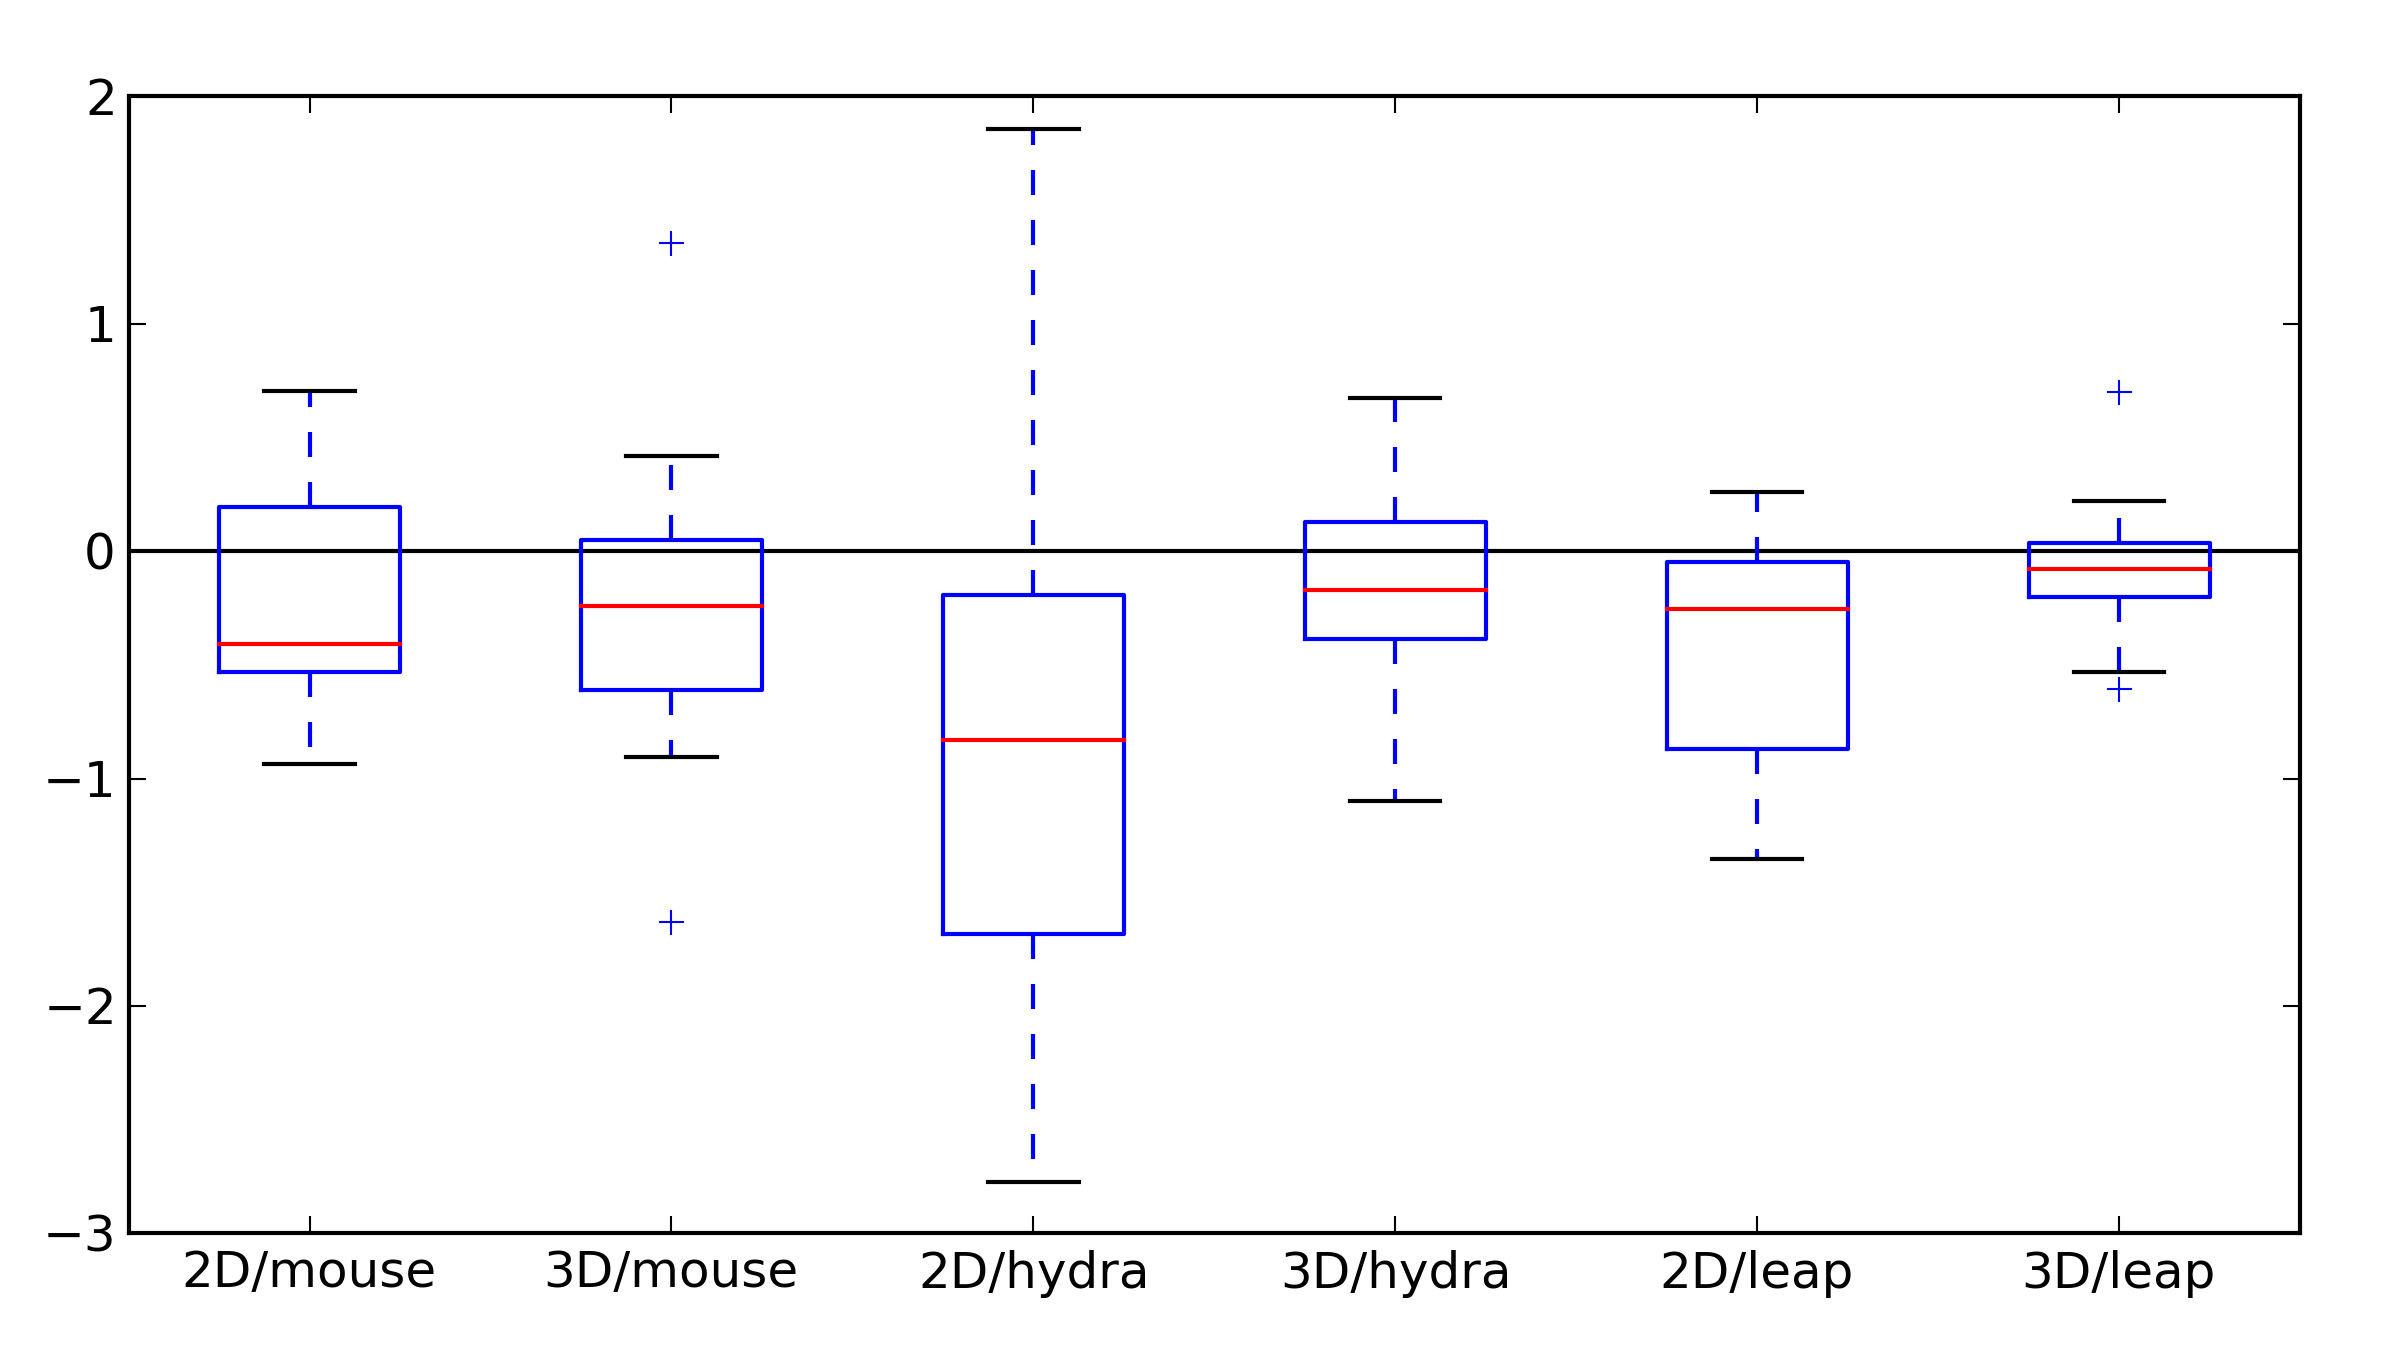
\includegraphics[width=\columnwidth]{improvement.png}
    \caption{Learning the inputs, reduction in completion time (s).}
    \label{fig:improvementtimes}
\end{figure}

\figref{deviation} plots the average perpendicular distance (deviation) from
the start-end target line segment for each subject for each input/output
modality.  A deviation of 0 would mean the cursor moved on a perfectly
straight path between the two targts.  We see there is significant inter
subject variance for the deviation, almost independent of input type.  For
example, subject 12 had the largest deviation for the mouse and keyboard / 2D
projections case, but one of the smaller for Leap / 3D headtracked.  The large
deviations in the Leap/ 3D headtracked case are mostly due to the Leap not
working correctly.

From the standpoint of adopting a new system in an organization,
\figref{fig:deviation} would indicate that some people will need extra time to
accustom themselves.  This extra time for familiarization should be taken into
account, e.g. by cautioning against getting frustrated right away.

\begin{figure}
  \centering
  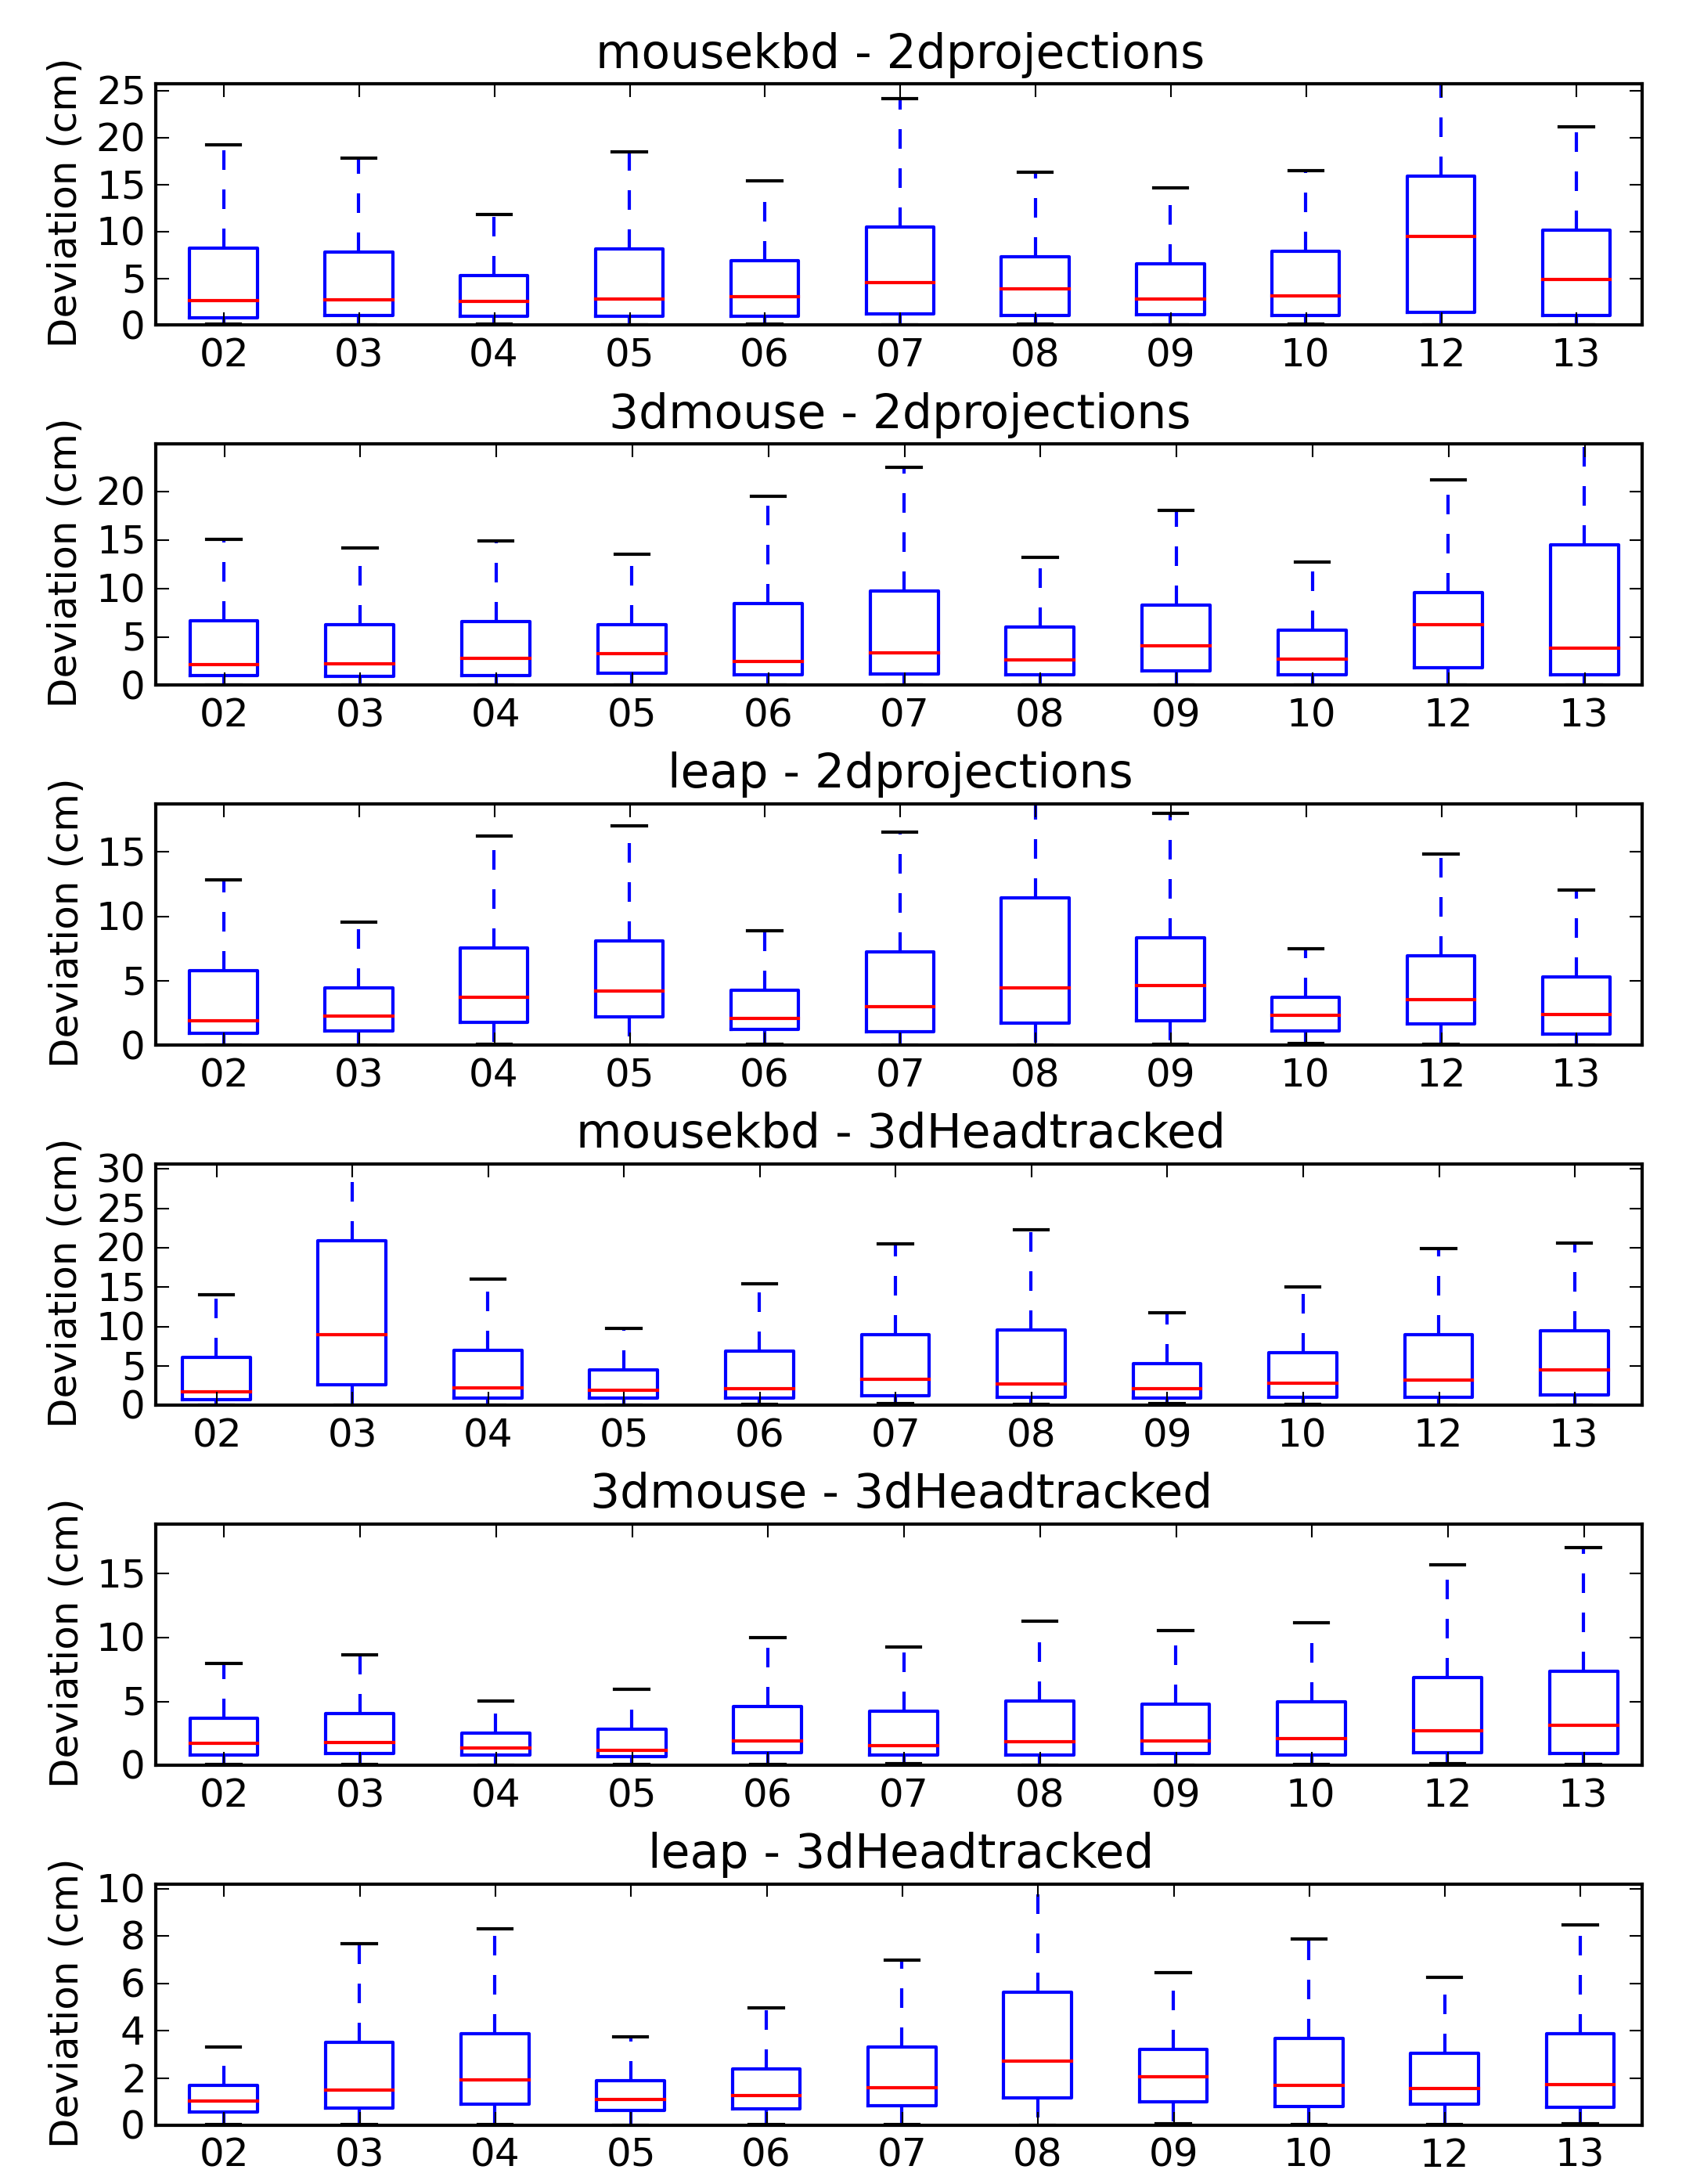
\includegraphics[width=\columnwidth]{deviation.png}
  \caption{Mean perpendicular distance from start-end line segment}
  \label{fig:deviation}
\end{figure}





\section{Discussion and Future Work}\label{sec:discussion}

Given the uniform distribution over prior 3D experience, we feel that our
results generalize at least to anyone with familiarity with computers.

Anecdote from \cite{leewii} about how parallax is really pretty immersing,
even if it is only approximately calibrated to head position.  Also the fact
that human ``steo'' vision is basically flat beyond 20 feet.  So, stereoscopic
displays are really only useful when interacting with objects at close range,
i.e. basically within arms reach, as our study did.

1-to-1 mapping as we implemented it requires a lot of setup (calibration process) and once done the components can't be moved.  This limits its ease of adoption in informal settings / at home / on laptops with 3d displays.

\subsection{User Feedback}\label{sec:feedback}

An important aspect of this experiment was to gather user feedback about their
impressions in using each modality; the most efficient interaction modality is
useless to implement if users dislike using it.  Feedback is also used to
suggest improvements to our system for future, larger scale testing.

On the whole, user feedback about our test system was very positive.  There
was very much a sense of the Wow! factor when using the full 3D systems,
despite its virtual wack-a-mole aspect, and several subjects commented that it
was fun in and of itself.

In the 3D output mode, subjects vastly preferred using the Hydra to the Leap
or mouse, even though the majority found the Leap to be the most intuitive
input, see \figref{fig:post}.  Based on their comments this is mainly due to
two factors: first, the Leap can be frustrating to use due to its imperfect
tracking (i.e. it either works well or horribly, no middle ground), and
second, that shoulder fatigure rapidly sets in, limiting the time for
comfortable interaction.  Another stated benefit of the Hydra was that its
relative motion allowed a user to reposition her hand without interrupting the
state of the workflow.

\begin{itemize}
\item ``[The Hydra] felt the most intuitive, and felt like it has the most
  potential for me to increase speed/precision over use.  The leap motion with
  3D viewing was a close second, but the fact that \emph{my hand occludes the
  display} during use was not too comfortable.''
\item ``Because [the Hydra] provides more accurate control and doesn't require
  too much effort to move. Leap motion is a pain for both cases, because it is
  always out of the detection range and it requires my arm to point to a
  precise location that is more tiring.''
\item ``The 3D headtracked monitor helped me see how close the object was to
  me. I liked the relative motion of the [Hydra]because it allowed me to
  reposition my hand and keep my arm in a comfortable range of motion.''
\end{itemize}

When asked about improvements to our system, a clear consensus was replacing the Leap with something more reliable.  Other suggested improvements involve the
UI design (include more graphical cues such as axes or cursor location
indicators) and improved 3D realism such as shading and shadows that
correspond with the physical environment.

\begin{figure}
    \centering
    \begin{tabular}{c | c | c}
    Favorite Combination & 2D & 3D \\ \hline
    Mouse and Keyboard   &    & 1 \\
    Hydra                &    & 9 \\
    Leap Motion          &    & 1 \\
    \end{tabular}

    \vspace{0.2in}

    \begin{tabular}{c | c | c}
    Most Intuitive     & 2D & 3D \\ \hline
    Mouse and Keyboard &    &  \\
    Hydra              &    & 4 \\
    Leap Motion        &    & 7 \\
    \end{tabular}

    \caption{Post-experiment responses}
    \label{fig:post}
\end{figure}



\section{Conclusion}\label{sec:conclusion}

This paper presented ...


% Balancing columns in a ref list is a bit of a pain because you
% either use a hack like flushend or balance, or manually insert
% a column break.  http://www.tex.ac.uk/cgi-bin/texfaq2html?label=balance
% multicols doesn't work because we're already in two-column mode,
% and flushend isn't awesome, so I choose balance.  See this
% for more info: http://cs.brown.edu/system/software/latex/doc/balance.pdf
%
% Note that in a perfect world balance wants to be in the first
% column of the last page.
%
% If balance doesn't work for you, you can remove that and
% hard-code a column break into the bbl file right before you
% submit:
%
% http://stackoverflow.com/questions/2149854/how-to-manually-equalize-columns-
% in-an-ieee-paper-if-using-bibtex
%
% Or, just remove \balance and give up on balancing the last page.
%
\balance

\bibliographystyle{acm-sigchi}
\bibliography{cse510}
\end{document}
